\item Given the conservation law $u_t + [\cos u]_x = 0$, sketch the characteristic curves, where
%
\begin{enumerate}
  \item
  $
  \displaystyle
  u(x, 0) =
  \begin{cases}
    \frac{\pi}{2} & x < 0\\
    0 & x \geq 0
  \end{cases}
  $

  \item
  $
  \displaystyle
  u(x, 0) =
  \begin{cases}
    \frac{\pi}{6} & x < 0\\
    \frac{\pi}{2} & x \geq 0
  \end{cases}
  $
\end{enumerate}

\bigbreak
%____________________________________________________________________________%

Here, we are given the conservation law. If we differentiate on $x$, we find:
%
\begin{align}
  u_t - u_x \sin u & = 0
\end{align}

  From here, let us use a third variable to solve our equation:
  %
  \begin{align}
    \frac{dt}{ds} & = 1\\
    \frac{dx}{ds} & = -\sin u\\
    \frac{du}{ds} & = 0
  \end{align}

  From here, we would let $t = s$.

\begin{enumerate}
    \item
  Here, we would want to consider $x(0) = x_0$ and $u(0) = f(x)$, which is given as $u(x, 0)$. If we make this assumption for $\frac{dx}{ds}$, we would get:
  %
  \begin{align}
    \frac{dx}{ds}
    & = - \sin u\\
    \frac{dx}{ds}
    & =
    \begin{cases}
      \sin \frac{\pi}{2} & x_0 < 0\\
      - \sin 0 & x_0 \geq 0
    \end{cases}
  \end{align}

  From here, if we evaluate our terms, we get:
  %
  \begin{align}
    \frac{dx}{ds} & =
    \begin{cases}
      -1 & x_0 < 0\\
      0 & p \geq 0
    \end{cases}
  \end{align}

  Now, if we multiply both sides by $ds$ and integrate, we would get:
  %
  \begin{align}
    x(s) & =
    \begin{cases}
      -s + x_0 & x_0 < 0\\
      x_0 & x_0 \geq 0
    \end{cases}
  \end{align}

  Here, recall $t = s$,
  %
  \begin{align}
    x(t) & =
    \begin{cases}
      -t + x_0 & x_0 < 0\\
      x_0 & x_0 \geq 0
    \end{cases}
  \end{align}

  \item
  Now, let us consider $u(x, 0)$ for part b) and write for $\frac{dx}{ds}$:
  %
  \begin{align}
    \frac{dx}{ds} & =
    \begin{cases}
      - \sin \frac{\pi}{6} & x_0 < 0\\
      - \sin \frac{\pi}{2} & x_0 \geq 0
    \end{cases}
  \end{align}

  When we integrate both sides with respect to their variables, we get:
  %
  \begin{align}
    x(s) & =
    \begin{cases}
      - 0.5 s + x_0 & x_0 < 0\\
      - s + x_0 & x_0 \geq 0
    \end{cases}\\
    x(t) & =
    \begin{cases}
      - 0.5 t + x_0 & x_0 < 0\\
      -     t + x_0 & x_0 \geq 0
    \end{cases}
  \end{align}

\end{enumerate}

Here are both characteristic lines plotted. Note that an extra line at
$x_0 = 0$ is added to show both equations at $x_0$:
%
\begin{center}
  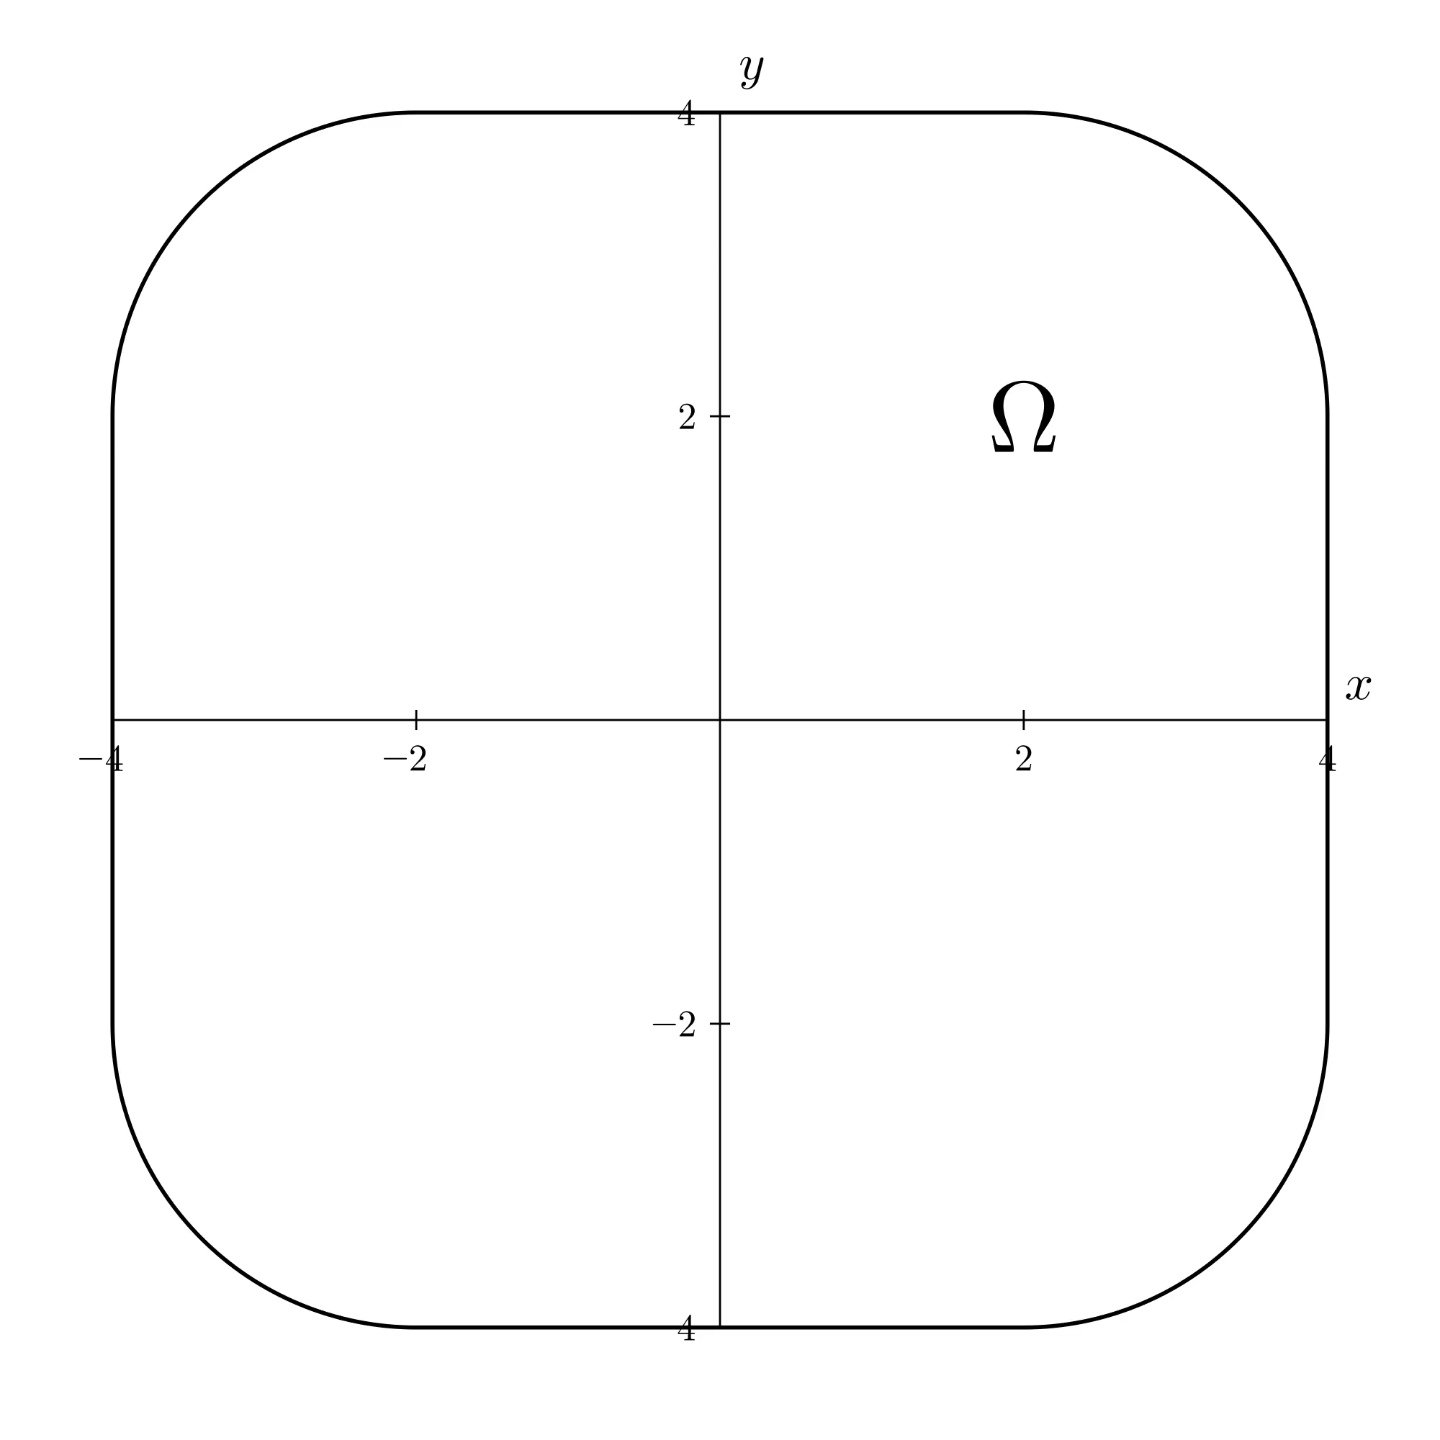
\includegraphics[height=4cm]{1a}
  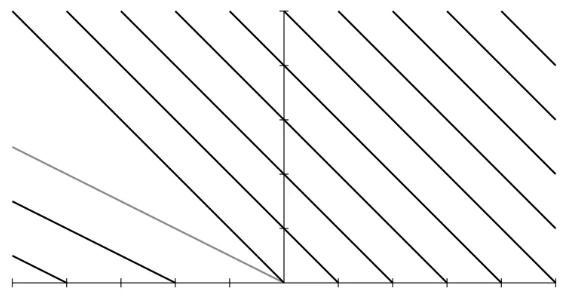
\includegraphics[height=4cm]{1b}
\end{center}
